% Created 2021-02-15 月 12:35
% Intended LaTeX compiler: pdflatex
\documentclass[presentation,dvipdfmx,CJKbookmarks]{beamer}
\usepackage{bxdpx-beamer}
\usepackage{CJKutf8}
\usepackage{atbegshi}
\AtBeginShipoutFirst{\special{pdf:tounicode UTF8-UTF16}} % for UTF-8
\usepackage[utf8]{inputenc}
\usepackage[T1]{fontenc}
\usepackage{graphicx}
\usepackage[export]{adjustbox}
\usepackage{lmodern}
\usepackage{grffile}
\usepackage{longtable}
\usepackage{wrapfig}
\usepackage{rotating}
\usepackage[normalem]{ulem}
\usepackage{amsmath}
\usepackage{textcomp}
\usepackage{amssymb}
\usepackage{capt-of}
\usepackage{hyperref}
 \usepackage{minted}
\usetheme{EastLansing}
\usecolortheme{default}

\date{2021-02-14}


\hypersetup{
 pdfauthor={包昊军},
 pdftitle={seL4\thinspace 介绍},
 pdfkeywords={},
 pdfsubject={},
 pdfcreator={Emacs 27.1 (Org mode 9.3)},
 pdflang={English}}
\begin{document}
\begin{CJK*}{UTF8}{simsun}

\title{seL4\thinspace 介绍}
\subtitle{\thinspace 一个被形式化验证的安全微内核}
\author{包昊军}

\maketitle
\begin{frame}{Outline}
\tableofcontents
\end{frame}

\CJKtilde

\section{seL4\thinspace 简介}
\label{sec:org4d831e3}
\begin{frame}[label={sec:org90830e8}]{微内核}
\begin{center}
\includegraphics[width=.9\linewidth]{./images/micro-kernel-structure.ps}
\end{center}
\end{frame}

\section{seL4\thinspace 项目}
\label{sec:org845ae00}
\begin{frame}[label={sec:orge8446d0}]{seL4\thinspace 官方项目}
\begin{itemize}
\item \href{https://docs.sel4.systems/projects/buildsystem/host-dependencies.html}{编译环境准备}
\end{itemize}
\begin{block}{sel4-tutorials(入门教程)}
\begin{description}
\item[{github}] \url{https://github.com/seL4/sel4-tutorials}
\item[{文档}] \url{https://docs.sel4.systems/Tutorials/}
\end{description}
\end{block}
\begin{block}{sel4test(unit tests and more)}
\begin{description}
\item[{github}] \url{https://github.com/seL4/sel4test}
\end{description}
\end{block}

\begin{block}{sel4-camkes(微内核嵌入式系统的组件化架构)}
\begin{description}
\item[{文档}] \url{https://docs.sel4.systems/projects/camkes/manual.html}
\end{description}
\end{block}
\end{frame}

\begin{frame}[label={sec:org71947c0}]{seL4\thinspace 社区项目}
\begin{block}{genode on sel4}
\begin{itemize}
\item 一个开源操作系统框架
\item sel4\thinspace 移植的过程写了\thinspace 3\thinspace 篇文章:\href{https://genode.org/documentation/articles/sel4\_part\_1}{1},\href{https://genode.org/documentation/articles/sel4\_part\_2}{2},\href{https://genode.org/documentation/articles/sel4\_part\_3}{3}
\end{itemize}
\end{block}
\begin{block}{\href{https://github.com/PolySync/cargo-fel4}{fel4}}
\begin{itemize}
\item 直接在\thinspace sel4\thinspace 上运行嵌入式\thinspace rust\thinspace 程序
\item 项目已过时,需要修改源码之后才能运行
\end{itemize}
\end{block}
\begin{block}{\href{https://gitlab.com/arm-research/security/icecap/icecap/}{icecap}}
\begin{itemize}
\item Arm Research\thinspace 的\thinspace sel4 rust\thinspace 项目
\end{itemize}
\end{block}
\end{frame}

\begin{frame}[label={sec:org40f3233}]{项目中使用组件框架的建议}
\begin{block}{seL4 API\thinspace 易用性差(重点在于形式化验证)}
\end{block}
\begin{block}{所以需要使用组件框架,重点关注业务逻辑}
\end{block}
\begin{block}{两个主要的组件框架:camkes\thinspace 和\thinspace genode}
\begin{itemize}
\item camkes\thinspace 主要用于静态系统:组件预定义,启动之后不再变化
\item genode\thinspace 更强大通用,但无法使用\thinspace sel4\thinspace 全部安全特性
\end{itemize}
\end{block}
\end{frame}

\section{sel4\thinspace 研究方向}
\label{sec:org4e04659}
\begin{frame}[label={sec:org45ec8b6}]{\href{https://ts.data61.csiro.au/students/theses.pml.html}{研究项目}}
\begin{itemize}
\item 多核、IPC\thinspace 性能优化
\item Secure, Android-based OS for IoT
\item seL4 AUTOSAR
\item Shared resources in an microkernel-based OS(用\thinspace camkes\thinspace 实现文件系统、网络协议栈)
\item Linux as a component(camkes-vm)
\end{itemize}
\end{frame}
\begin{frame}[label={sec:org7fc68f6}]{\href{https://github.com/seL4/docs/blob/master/SuggestedProjects.md}{Github\thinspace 项目建议}}
\begin{itemize}
\item 移植\thinspace minix3\thinspace 到\thinspace sel4
\end{itemize}
\end{frame}

\section{sel4\thinspace 动态}
\label{sec:org331d134}
\begin{frame}[label={sec:orgdde232d}]{sel4\thinspace 动态}
\begin{itemize}
\item 2020\thinspace 年\thinspace 4\thinspace 月,成立\thinspace seL4\thinspace 基金会,由\thinspace Linux\thinspace 基金会托管(\href{https://microkerneldude.wordpress.com/2020/04/07/the-sel4-foundation-what-and-why/}{sel4\thinspace 原作者博客})
\item 2021\thinspace 年\thinspace 2\thinspace 月,FOSDEM 2021
\end{itemize}
\end{frame}
\begin{frame}[label={sec:org8901b3d}]{sel4 RFC}
\begin{center}
\includegraphics[width=.9\linewidth]{./images/rfc-for-core.ps}
\end{center}
\begin{itemize}
\item Core、Core Platform
\end{itemize}
\end{frame}

\begin{frame}[label={sec:org7ba95ea}]{sel4 multi-server OS}
\begin{center}
\includegraphics[width=.9\linewidth]{./images/multi-server.os.ps}
\end{center}
\end{frame}

\begin{frame}[label={sec:org42cd3cd}]{sel4 multi-server OS}
\begin{center}
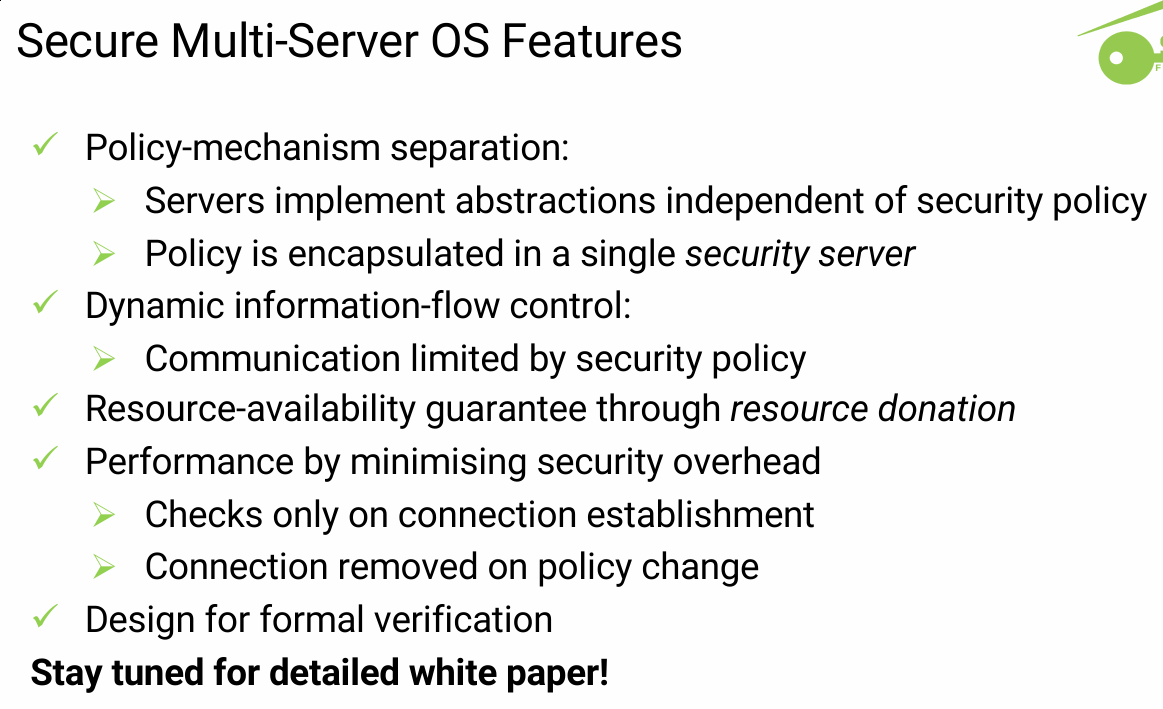
\includegraphics[width=.9\linewidth]{./images/multi-server.os.2.ps}
\end{center}
\end{frame}
\section{参考链接}
\label{sec:org4a0dc7d}
\begin{frame}[label={sec:orgcd16e74}]{参考链接}
\begin{itemize}
\item \href{https://sel4.systems/About/seL4-whitepaper.pdf}{白皮书}
\end{itemize}
\end{frame}
\end{CJK*}
\end{document}
